\clearpage
\VerdierPhysicalPageAnchor{0056}%
\VerdierSemanticAnchor{ch1-1-5-6}
\noindent\textbf{図式 1.5.6.}\quad
次に主張 (1.5.4.3) を証明しよう。証明は次の図式に基づく。
簡単のため、遷移同型 $c,c'$ が恒等射である場合について書く：

\VerdierSemanticAnchor{ch1-1-5-7}
\noindent\textbf{1.5.7.}

\VerdierSemanticAnchor{ch1-1-5-7-diagram}
\begin{center}
  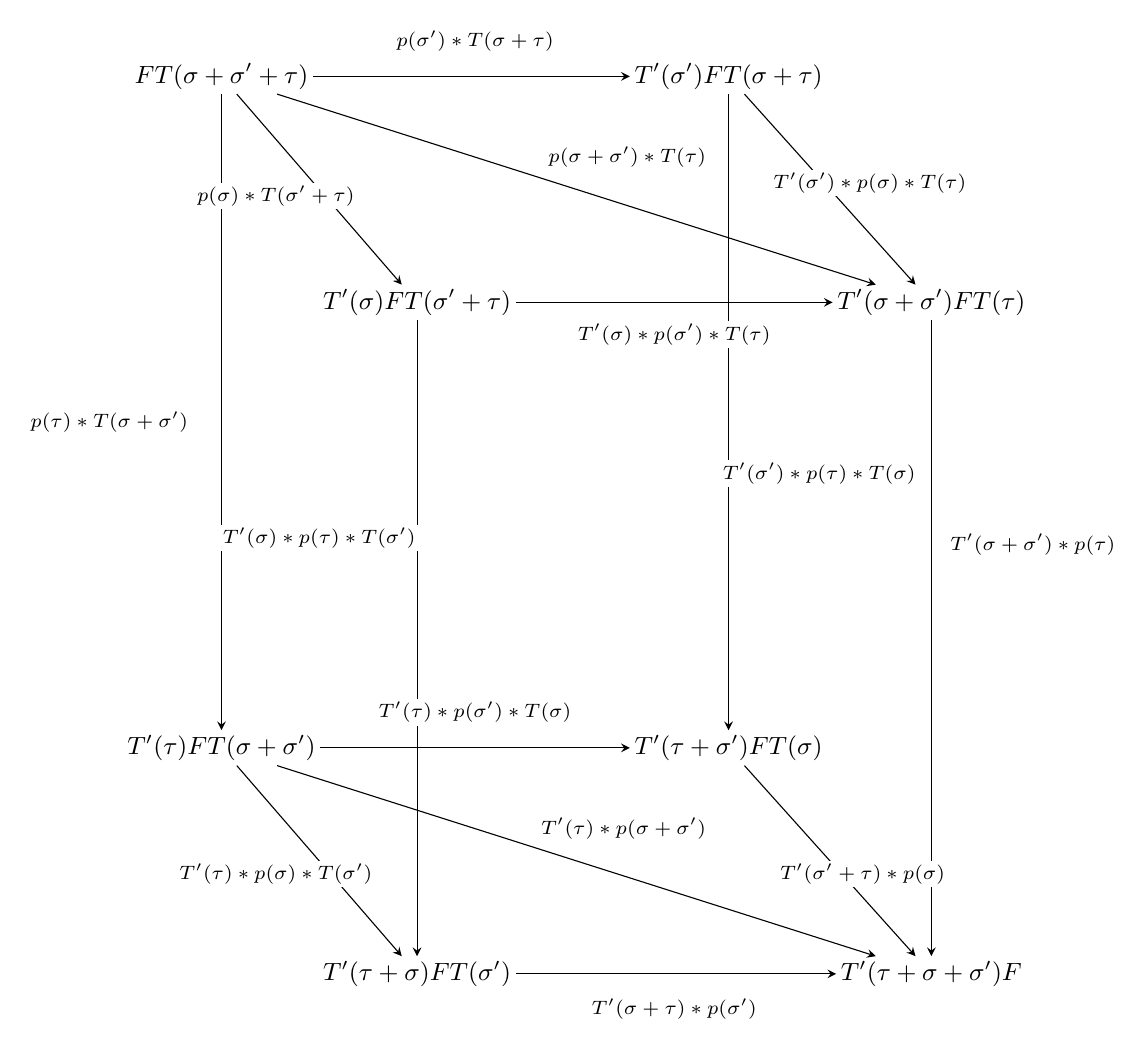
\begin{tikzpicture}[x=.92cm,y=.82cm,>=stealth,
      object/.style={inner sep=1.5pt,font=\small},
      lab/.style={font=\scriptsize,fill=white,inner sep=1pt}]
    \node[object] (a) at (-5.8,13.0) {$FT(\sigma+\sigma'+\tau)$};
    \node[object] (b) at (1.2,13.0) {$T'(\sigma')FT(\sigma+\tau)$};
    \node[object] (c) at (-3.1,9.5) {$T'(\sigma)FT(\sigma'+\tau)$};
    \node[object] (d) at (4.0,9.5) {$T'(\sigma+\sigma')FT(\tau)$};
    \node[object] (e) at (-5.8,2.6) {$T'(\tau)FT(\sigma+\sigma')$};
    \node[object] (f) at (1.2,2.6) {$T'(\tau+\sigma')FT(\sigma)$};
    \node[object] (g) at (-3.1,-0.9) {$T'(\tau+\sigma)FT(\sigma')$};
    \node[object] (h) at (4.0,-0.9) {$T'(\tau+\sigma+\sigma')F$};

    \draw[->] (a) -- (b);
    \draw[->] (a) -- (c);
    \draw[->] (a) -- (d);
    \draw[->] (a) -- (e);
    \draw[->] (b) -- (d);
    \draw[->] (b) -- (f);
    \draw[->] (c) -- (d);
    \draw[->] (c) -- (g);
    \draw[->] (d) -- (h);
    \draw[->] (e) -- (f);
    \draw[->] (e) -- (g);
    \draw[->] (e) -- (h);
    \draw[->] (f) -- (h);
    \draw[->] (g) -- (h);

    \node[lab] at (-2.3,13.55) {$p(\sigma')*T(\sigma+\tau)$};
    \node[lab] at (-5.05,11.15) {$p(\sigma)*T(\sigma'+\tau)$};
    \node[lab] at (-0.2,11.75) {$p(\sigma+\sigma')*T(\tau)$};
    \node[lab] at (-7.35,7.65) {$p(\tau)*T(\sigma+\sigma')$};
    \node[lab] at (3.15,11.35) {$T'(\sigma')*p(\sigma)*T(\tau)$};
    \node[lab] at (2.45,6.85) {$T'(\sigma')*p(\tau)*T(\sigma)$};
    \node[lab] at (0.45,9.00) {$T'(\sigma)*p(\sigma')*T(\tau)$};
    \node[lab] at (-4.45,5.85) {$T'(\sigma)*p(\tau)*T(\sigma')$};
    \node[lab] at (5.40,5.75) {$T'(\sigma+\sigma')*p(\tau)$};
    \node[lab] at (-2.3,3.15) {$T'(\tau)*p(\sigma')*T(\sigma)$};
    \node[lab] at (-5.05,0.65) {$T'(\tau)*p(\sigma)*T(\sigma')$};
    \node[lab] at (-0.25,1.35) {$T'(\tau)*p(\sigma+\sigma')$};
    \node[lab] at (3.05,0.65) {$T'(\sigma'+\tau)*p(\sigma)$};
    \node[lab] at (0.45,-1.45) {$T'(\sigma+\tau)*p(\sigma')$};
  \end{tikzpicture}
\end{center}

\VerdierSemanticAnchor{ch1-1-5-7-delta-intro}
$\Delta(\sigma,\tau)$ を図式
$\textup{(1.5.4.2)}_{\sigma,\tau}$ とする。上の図式は
